\documentclass{report}
%Configuration page
\usepackage{geometry}
\geometry{
	width=21.59cm, 
	height=27.94cm,
	left=3.17cm,
	right=3.81cm,
	bottom=3.81cm,
	top=3.17cm,
}

%...............................................................
%Tamaño para titulos de chapters,secciones,subsecciones
\usepackage{sectsty}
\usepackage{titlesec}
\sectionfont{\large}
\subsectionfont{\large}
%...............................................................
%figures and Tables 
\usepackage{caption}
\usepackage{subcaption}
%...............................................................
%Using Packages (general)
\usepackage[utf8]{inputenc}
\usepackage[T1]{fontenc, url}
\usepackage[spanish,es-tabla]{babel}
\usepackage{times} %Use Font Times New Roman 
\usepackage{amsmath}
\usepackage{amsfonts}
\usepackage{amssymb}
\usepackage{makeidx}
\usepackage{graphicx}
\graphicspath{{figures/}} %Import images from folder
\usepackage{float}
\usepackage[table,xcdraw]{xcolor}
\usepackage[toc,page]{appendix}
%...............................................................
%Comments
\usepackage{comment}%Comments in file  
\usepackage[colorinlistoftodos]{todonotes}%Comments in pdf
%...............................................................
%Generic text packages 
\usepackage{blindtext}
\usepackage{lipsum}
%...............................................................
%Change tables, contents, figures parameters 
\usepackage{tocloft}
\usepackage{tocenter}
\usepackage{gensymb} %Degree Symbol
\usepackage{textcomp} %Symbols 
\usepackage{chngpage}% allows for temporary adjustment of side margins
%...............................................................
%Page style
\usepackage{fancyhdr}
\pagestyle{fancy}
\fancyhf{}
\lhead{Pontificia Universidad Javeriana}
\rhead{Memoria de Trabajo de Grado - Profundización}
\rfoot{Página \thepage}
\renewcommand{\headrulewidth}{0.5pt}
\renewcommand{\footrulewidth}{0.5pt}
%...............................................................
%Redefine plain (chapters, tables, appendix)
\fancypagestyle{plain}{
\fancyhf{}
\fancyhead[OL]{Pontificia Universidad Javeriana}
\fancyhead[OR]{Memoria de Trabajo de Grado - Profundización}
\fancyfoot[R]{Página \thepage}
\fancyfoot[L]
}
%...............................................................
% To make cites and references
\usepackage[hidelinks,pdfusetitle,pdfdisplaydoctitle]{hyperref} 
\usepackage{doi}
\renewcommand{\doitext}{}
\usepackage{natbib} %Package to cite references
%...............................................................
% To make pretty tables
\usepackage{booktabs}
\usepackage{multirow}
\usepackage{dcolumn}
\usepackage{array}
%Control de terminaciones de linea en párrafo
\hyphenpenalty=100000   % No se dividen las palabras al terminar una línea
\sloppy % Ayuda a que las cosas no se salgan de los márgenes.
\raggedbottom % Hace que el tamaño de las páginas llegue hasta donde llegue el texto, no agrega espacio vertical

%----------------------------------------------------------------------------%
\begin{document}

    \thispagestyle{empty}
\newcommand{\CODIGOTG}{12345}
\newcommand{\TITULOTG}{ Evaluación e implementación de métodos de extracción automática de palabras clave aplicados a textos cortos en español}
\newcommand{\AUTORESTG}{Kelly Gisselle Candelo\\
Andrea Guti{\'e}rrez Ladino\\
Iv{\'a}n Felipe Molano}
\newcommand{\DIRECTORTG}{Alexandra Pomares Quimbaya}

\begin{center}
	%\vspace{0.1cm}
		\vspace*{2cm}
		\fontsize{16pt}{16pt}\textbf{\CODIGOTG\ }\\
		\fontsize{14pt}{14pt}\selectfont \TITULOTG\ \\ %Modificar de acuerdo a la facultad
%............................................................................	
		\vspace*{5cm}
		\fontsize{14pt}{14pt}\selectfont Autores\\
		\AUTORESTG\ \\
		%Debajo del título con 
%............................................................................
		\vspace*{5cm}
		\fontsize{14pt}{14pt}\selectfont PONTIFICIA UNIVERSIDAD JAVERIANA\\
		FACULTAD DE INGENIERIA\\
		MAESTRÍA EN INGENIERÍA DE DE SISTEMAS Y COMPUTACIÓN\\
		BOGOTÁ, D.C.\\
		2021 
\end{center}


    \thispagestyle{empty}

\begin{center}

		\fontsize{12pt}{12pt}\textbf{<CÓDIGO>}\\
		\fontsize{14pt}{14pt}\selectfont Título del Trabajo de Grado\\ %Modificar de acuerdo a la facultad
%............................................................................	
		\vspace*{3cm}
		\fontsize{12pt}{12pt}\textbf{Autor:}\\ 
		\vspace{0.2cm}
		\fontsize{14pt}{14pt}Nombre Completo del Autor\\
%............................................................................
        \vspace*{4cm}
		\fontsize{12pt}{12pt}{MEMORIA DEL TRABAJO DE GRADO REALIZADO PARA CUMPLIR UNO DE LOS REQUISITOS PARA OPTAR AL TITULO DE MAGÍSTER EN INGENIERÍA DE SISTEMAS Y COMPUTACIÓN}

%............................................................................
        \vspace*{1.7cm}
		\fontsize{12pt}{12pt}\textbf{Directora}\\
		\vspace{0.2cm}
        Nombre completo del director del TG\\
        \vspace{0.2cm}
        \textbf{Comité de Evaluación del Trabajo de Grado}\\
        \vspace{0.2cm}
        <Nombres y Apellidos Completos del Jurado >\\
        \vspace{0.2cm}
        <Nombres y Apellidos Completos del Jurado >\\
        \vspace{0.2cm}
        \textbf{Página web del Trabajo de Grado}\\
        \vspace{0.2cm}
        http://pegasus.javeriana.edu.co/~<código>\\
%............................................................................

		\vspace*{1.8cm}
		\fontsize{12pt}{12pt}\selectfont PONTIFICIA UNIVERSIDAD JAVERIANA\\
		FACULTAD DE INGENIERIA\\
		MAESTRÍA EN INGENIERÍA DE DE SISTEMAS Y COMPUTACIÓN\\
		BOGOTÁ, D.C.\\
		<MES><AÑO> %Modificar de acuerdo al año vigente
\end{center}
    \thispagestyle{empty}

\begin{center}

		\fontsize{12pt}{12pt}\textbf{PONTIFICIA UNIVERSIDAD JAVERIANA\\
		FACULTAD DE INGENIERIA\\
		MAESTRÍA EN INGENIERÍA DE SISTEMAS Y COMPUTACIÓN}\\
%............................................................................	
        \vspace*{10cm}
		\fontsize{12pt}{12pt}\selectfont \textbf{Rector Magnífico}\\
		\vspace{0.2cm}
        Jorge Humberto Peláez, S.J.\\
        \vspace{0.2cm}
        \textbf{Decano Facultad de Ingeniería}\\
        \vspace{0.2cm}
        Ingeniero Lope Hugo Barrero Solano\\
        \vspace{0.2cm}
        \textbf{Director Maestría en Ingeniería de Sistemas y Computación}\\
        \vspace{0.2cm}
        Ingeniera Angela Carrillo Ramos\\
        \vspace{0.2cm}
        \textbf{Director Departamento de Ingeniería de Sistemas}\\
        \vspace{0.2cm}
        Ingeniero Efraín Ortíz Pabón\\
        
\end{center}
    \setcounter{page}{4}
%..................................	
	%Sections 
	\begin{flushleft}
		\phantomsection \label{artículo}
		\vspace*{2cm}
		\large{\textbf{Artículo 23 de la Resolución No. 1 de Junio de 1946}}
	\end{flushleft}
	\input{Resolución}
	\clearpage

%..................................	
	%Sections 
	\begin{center}
		\phantomsection \label{glads}
		\large{\textbf{AGRADECIMIENTOS}}
	\end{center}
	\fontsize{11pt}{11pt}\selectfont %Cambiar si se desea letra más grande
\vspace*{0.2cm}
Escribir un mensaje en caso de que sienta agradecimiento por alguien que lo haya apoyado en el desarrollo del Trabajo de Grado. Su fami-lia, su pareja, sus amigos, su director, sus profesores, etc\\
	\clearpage
%..................................	
    %\fontsize{11pt}{11pt}\selectfont %Cambiar si se desea letra más grande 
\vspace*{0.2cm}
\begin{center}
    \fontsize{14pt}{14pt}\textbf{ABSTRACT}\\
\end{center}
\vspace*{0.2cm}
\noindent Write a paragraph in English in which a reader could understand what the problem was and what you have done to resolve it. Maximum 100 words.  You can support this activity by reading the information that you can find in the following hyperlinks:
%-----------------------------------------------------------------------------
\vspace*{1.5cm}
\begin{center}
    \fontsize{14pt}{14pt}\textbf{RESUMEN}\\
\end{center}
\vspace*{0.2cm}
\noindent Escriba un párrafo en el cual un lector pueda entender cuál fue el problema y qué se hizo para resolverlo. Máximo 100 palabras. Usted puede utilizar la información contenida en los siguientes enlaces para escribir un buen abstract o resumen:

%..................................	
    \begin{center}
		\phantomsection \label{resumenejecutivo}
		\large{\textbf{RESUMEN EJECUTIVO}}
	\end{center}
	\fontsize{11pt}{11pt}\selectfont %Cambiar si se desea letra más grande 
\vspace*{0.5cm}
Describa brevemente la problemática, diga lo que se hizo y presente los resultados y conclu-siones principales que se obtuvieron con su realización. Mínimo 1000 palabras, máximo 1200.
	\clearpage

%..................................	
    \setlength{\cftbeforetoctitleskip}{-0.3cm}
	\renewcommand{\cfttoctitlefont}{\large}
	\renewcommand{\contentsname}{\textbf{CONTENIDO}}
	
	\tableofcontents 
	\newpage
	\renewcommand\cftloftitlefont{\large}
	\renewcommand{\listfigurename}{\textbf{ÍNDICE DE FIGURAS}}
	%\listoffigures
	{%
		\let\oldnumberline\numberline%
		\renewcommand{\numberline}{\figurename~\oldnumberline}%
		\listoffigures%
	}
	\newpage
	\renewcommand\cftlottitlefont{\large}
	\renewcommand{\listtablename}{\textbf{ÍNDICE DE TABLAS}}
	{%
		\let\oldnumberline\numberline%
		\renewcommand{\numberline}{\tablename~\oldnumberline}%
		\listoftables%
	}
	\newpage
%..................................	
	%\pagenumbering{arabic} % Comienza la numeración arábiga (números normales)
	%\setcounter{page}{1} % Comienza el contador de páginas en 1
%..................................	
	\chapternumberfont{\huge}
	\chaptertitlefont{\large}
	\chapter{INTRODUCCIÓN} \label{intr}
	\fontsize{14}{15}\selectfont
\section{Caso de estudio}
\lipsum[1]\\
\section{Planteamiento del Problema}
\lipsum[1]\\
\section{Objetivos}
\subsection{Objetivo General}
\begin{itemize}
	\item Determinar la condición física de los alumnos de la Carrera de Geología de la UCN.
\end{itemize}
\subsection{Objetivos Específicos}
\begin{enumerate}
	\item Identificar los lineamientos o posibles fallas en el área de estudio. 
	\item Establecer marcadores morfológicos para la conocer su cinemática.
	\item Determinar tipo de movimiento y/o características tienen los rasgos estructurales del área.
\end{enumerate}
\section{Ubicación del área de estudio}
El área de captación por las técnicas ocupadas (InSAR y GPS), pueden abarcar aún más territorio hacia el norte, sur, y este de la península, llegando a ser cerca de 27.000 km$^2$ (Figura \ref{ilustracion1}).\\
\begin{figure}[hb]
	\centering
	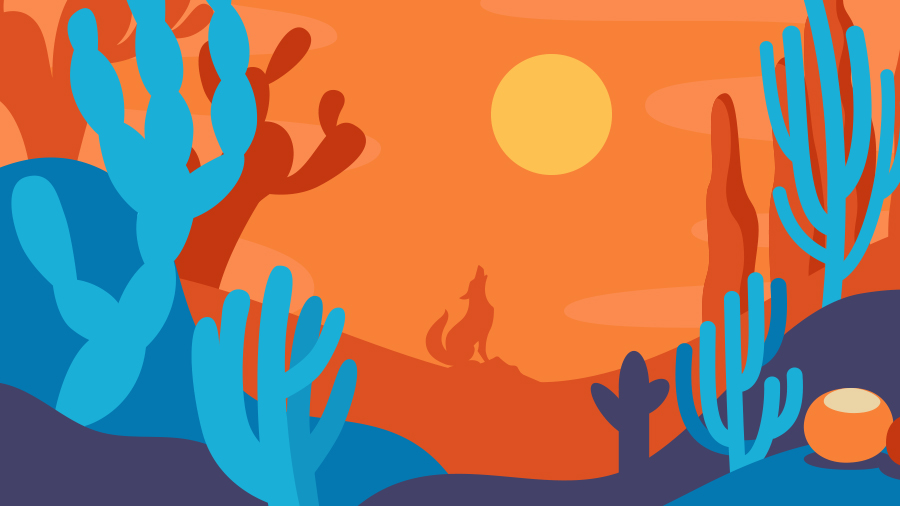
\includegraphics[scale=0.4]{figure1.jpg} %Change the figure name 
	\setstretch{1} %Interlineado 1
	\captionsetup{labelsep=period, labelfont=bf}
	\caption[Ilustración zorro en desierto]{\blindtext[1]} %[Se muestra en el índice]{Se muestra en el pie de figura}
	\label{ilustracion1}
\end{figure}



\section{Data y Metodología}
\lipsum[1]
%..................................	
	\chapter{MARCO TEÓRICO} \label{cap2}
	\fontsize{14}{15}\selectfont
\section{Interferometría de radar de apertura sintética (InSAR)}
\blindtext\\

\blindtext\\

En la Figura \ref{ilustracion2} se muestra el cuadro representativo de una palta simulando una mochila, etc etc etc.\\

\begin{figure}[h]
	\centering
	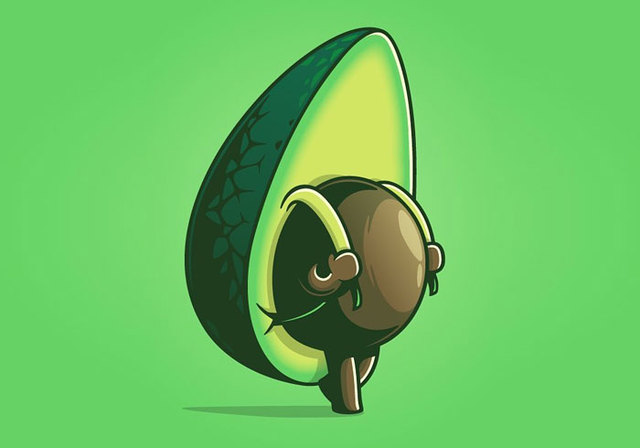
\includegraphics[scale=0.6]{figure3.jpg} %Change the figure name 
	\setstretch{1} %Interlineado 1
	\captionsetup{labelsep=period, labelfont=bf}
	\caption[Ilustración zorro en desierto]{\blindtext[1]} %[Se muestra en el índice]{Se muestra en el pie de figura}
	\label{ilustracion2}
\end{figure}

%..................................	
	\chapter{MARCO TEÓRICO 2} \label{cap3}
	\fontsize{14}{15}\selectfont
\blindtext\\

\section{Modelo numérico}
\blindtext
% Listado de puntos 
\begin{itemize}
	\item Punto1.
	\item Punto2.
	\item Punto3.
	\item Punto4.
	\item Punto5.
	\item Punto6.
	\item Punto7 \citep{allmendinger_invited_2010}. %Ejemplo de cita conectada con un bibtex
\end{itemize}
%..................................	
	\chapter{MARCO GEOLÓGICO}
	\fontsize{14}{15}\selectfont
Chile se encuentra situado a lo largo de un margen convergente, en el cual la placa de Nazca se subduce por debajo de la placa Sudamericana, con una convergencia oblicua con orientación N75°E, a una velocidad de $\sim$ 6.7 cm/año \citep*{angermann_space-geodetic_1999,argus_geologically_2011}. Según \cite{bejar-pizarro_asperities_2010} el terremoto de Tocopilla 2007 etc etc etc. La ecuación \eqref{eq:1} es un ejmeplo para realizar una ecuación correctamente.\\
\begin{equation}
	\Delta \Phi_{flat,topo,defo} = \dfrac{4\pi}{\lambda}\cdot\Delta R
	\label{eq:1}
\end{equation}\\
Para matrices realizar la ecuación \eqref{eq:matrix}:\\
\begin{equation}
	\Delta L= \begin{bmatrix}
		sen(\theta)\cdot sen(\alpha) & -sen(\theta)\cdot cos(\alpha) & cos(\theta)
	\end{bmatrix}
	\begin{bmatrix}
		\delta Norte\\
		\delta Este\\
		\delta Up\\
	\end{bmatrix}
	\label{eq:matrix}
\end{equation}\\
%..................................	
	\chapter{RESULTADOS}
	\fontsize{14}{15}\selectfont
\section{Resultado 1}
\blindtext\\
\section{Resultado 1}
\blindtext
%..................................	
	\chapter{DISCUSIÓN}
	\fontsize{14}{15}\selectfont
\blindtext
%............Table:style1.........................%
\begin{table}[h]
    \begin{tabular}{  l  p{3cm}  p{7.7cm} } %Ir probando con estos números 
        \toprule
\textbf{Investigación}      
& \textbf{Interpretación}   
& \textbf{Características} \\\midrule
Investigación 1
& It is only possible to represent aspects of social reality. Researcher is a subjective observer. The world is open to interpretation.        
& The world is characterised by inequalities because the lifeworld is systemically colonised. Ideology is all-pervasive. Knowledge implies action. \\\hline
Investigación 2       
& Engage with other people’s lives Enable the ‘voices’ of others to be heard                         
& Critically observe design practices Engage with other people’s lives Initiate or facilitate change  \\\hline
Investigación 3        
& To explore the habitus of designers and users, in,interaction with the field To interpret design practices, objects and systems To understand how the designer or the user engages with design practices, objects and systems 
& To disrupt, emancipate, transform the habitus and field of design To explore how the user is affected by design practices, objects and systems To change design practices, \\
    \bottomrule
    \end{tabular}
    \captionsetup{labelsep=period, labelfont=bf}
    \caption{Interpretación y característica generales de cada investigación constituida.}
     \label{table1}
\end{table}
%............................................%
%..................................	
	\chapter{CONCLUSIÓN}
	\fontsize{14}{15}\selectfont
\blindtext
	\clearpage
%..................................	
	\addcontentsline{toc}{chapter}{REFERENCIAS}
	\renewcommand{\bibname}{REFERENCIAS}
	\bibliographystyle{apalike}
	\setstretch{1}
	\setlength{\bibsep}{2em plus 0.5ex}
	\bibliography{references/papers} %Link a referencias
	\clearpage
%..................................	
	\appendix
	\renewcommand{\appendixname}{ANEXOS}
	\renewcommand{\appendixpagename}{ANEXOS}
	\renewcommand{\appendixtocname}{ANEXOS}
	\addappheadtotoc	
	\fontsize{12pt}{14.5}\selectfont
\chapter{Tablas y gráficos de conexión} \label{anexo1}
\section{Tablas Series de Tiempo}
%............Table:style2.........................%
\begin{table}[ht]
	\centering
	\setlength{\arrayrulewidth}{1mm}
	\renewcommand{\arraystretch}{2.5}
	\arrayrulecolor{white}
	\begin{tabular}{|l|l|l|l|l|l|}
		\hline
		\rowcolor[HTML]{E0E0E0} 
		{\color[HTML]{000000} \textbf{Ciudad}} & {\color[HTML]{000000} \textbf{Número}} & {\color[HTML]{000000} \textbf{Edificio 1}} & {\color[HTML]{000000} \textbf{Remodelación 1}} & {\color[HTML]{000000} \textbf{Valor[millones]}} & {\color[HTML]{000000} \textbf{Tiempo}} \\ \hline
		\rowcolor[HTML]{EFEFEF} 
		{\color[HTML]{000000} París}               & {\color[HTML]{000000} 361}           & {\color[HTML]{000000} 11 Ago 2007}         & {\color[HTML]{000000} 24 Nov 2007}         & {\color[HTML]{000000} $\sim$135}            & {\color[HTML]{000000} 105 días}            \\ \hline
		\rowcolor[HTML]{EFEFEF} 
		{\color[HTML]{000000} New York}              & {\color[HTML]{000000} 368}           & {\color[HTML]{000000} 10 Oct 2007}         & {\color[HTML]{000000} 24 Nov 2007}         & {\color[HTML]{000000} $\sim$259}            & {\color[HTML]{000000} 35 días}             \\ \hline
		\rowcolor[HTML]{EFEFEF} 
		{\color[HTML]{000000} Zurich}              & {\color[HTML]{000000} 96}            & {\color[HTML]{000000} 05 Nov 2007}         & {\color[HTML]{000000} 10 Dic 2007}         & {\color[HTML]{000000} $\sim$-204 }            & {\color[HTML]{000000} 35 días}             \\ \hline
	\end{tabular}
	\label{table:1anexo1}
\end{table}
%............................................%
\newpage %Cambiar de página
\section{Gráficos de Conexión}
\chapter{Lugares extras} \label{anexo2}
\section{Lugar extra 1}
\begin{figure}[h]
	\centering
	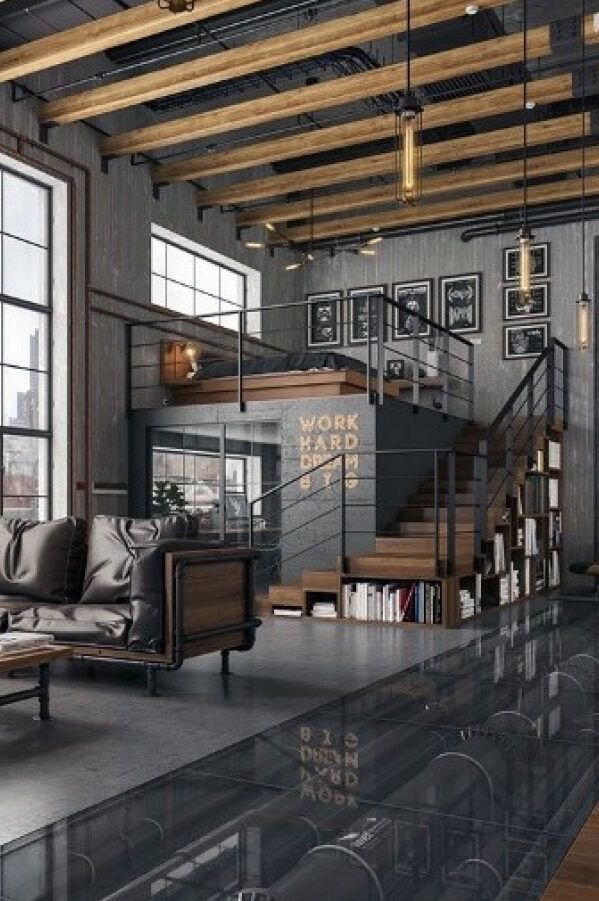
\includegraphics[scale=0.4]{figure4} 
	\label{ilustracion4} 
\end{figure}

\end{document}
